% !TEX TS-program = pdflatex
% !TEX encoding = UTF-8 Unicode

% This is a simple template for a LaTeX document using the "article" class.
% See "book", "report", "letter" for other types of document.

\documentclass[11pt]{report} % use larger type; default would be 10pt

\usepackage[utf8]{inputenc} % set input encoding (not needed with XeLaTeX)

%%% Examples of Article customizations
% These packages are optional, depending whether you want the features they provide.
% See the LaTeX Companion or other references for full information.

%%% PAGE DIMENSIONS
\usepackage{geometry} % to change the page dimensions
\geometry{a4paper} % or letterpaper (US) or a5paper or....
% \geometry{margin=2in} % for example, change the margins to 2 inches all round
% \geometry{landscape} % set up the page for landscape
%   read geometry.pdf for detailed page layout information

\usepackage{graphicx} % support the \includegraphics command and options

% \usepackage[parfill]{parskip} % Activate to begin paragraphs with an empty line rather than an indent

%%% PACKAGES
\usepackage{booktabs} % for much better looking tables
\usepackage{array} % for better arrays (eg matrices) in maths
\usepackage{paralist} % very flexible & customisable lists (eg. enumerate/itemize, etc.)
\usepackage{verbatim} % adds environment for commenting out blocks of text & for better verbatim
\usepackage{subfig} % make it possible to include more than one captioned figure/table in a single float
% These packages are all incorporated in the memoir class to one degree or another...

%%% HEADERS & FOOTERS
\usepackage{fancyhdr} % This should be set AFTER setting up the page geometry
\pagestyle{fancy} % options: empty , plain , fancy
\renewcommand{\headrulewidth}{0pt} % customise the layout...
\lhead{}\chead{}\rhead{}
\lfoot{}\cfoot{\thepage}\rfoot{}

%%% SECTION TITLE APPEARANCE
\usepackage{sectsty}
\allsectionsfont{\sffamily\mdseries\upshape} % (See the fntguide.pdf for font help)
% (This matches ConTeXt defaults)

%%% ToC (table of contents) APPEARANCE
\usepackage[nottoc,notlof,notlot]{tocbibind} % Put the bibliography in the ToC
\usepackage[titles,subfigure]{tocloft} % Alter the style of the Table of Contents
\renewcommand{\cftsecfont}{\rmfamily\mdseries\upshape}
\renewcommand{\cftsecpagefont}{\rmfamily\mdseries\upshape} % No bold!

\usepackage{hyperref}
\usepackage{graphicx} 
\usepackage[labelformat=empty]{caption}
\usepackage{pstricks}

%%% END Article customizations

%%% The "real" document content comes below...

\title{Confronto tra Pig e Java MapReduce}
\author{Enrico Giordano VR386687}
%\date{} % Activate to display a given date or no date (if empty),
         % otherwise the current date is printed 

\begin{document}

\begin{titlepage}
    \centering
    \vfill
    {\bfseries\Large
        Confronto tra Pig e Java MapReduce\\
        \vskip2cm
        Enrico Giordano VR386687\\
    }    
    \vfill
    \begin{figure}[htbp]
    \centering
    	\fbox{
	    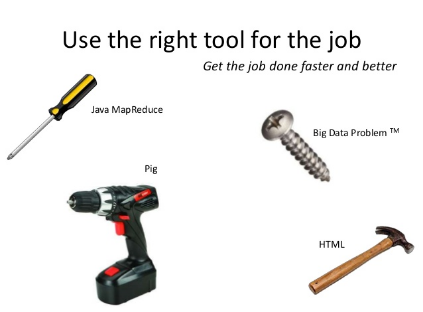
\includegraphics{pigmapreduce.png}
	 }
    	\caption{Donald Miner, NYC Data Science Meetup on “Hadoop for Data Science”}
    \end{figure}
     \vfill
    \vfill
\end{titlepage}

\newpage 

\section{Introduzione}

Questo progetto ha lo scopo di confrontare due diverse tecnologie utilizzate nell'ambito dei sistemi per elaborazione di grandi quantità di dati, ovvero un linguaggio di scripting chiamato ``Pig'' e un framework basato su Java chiamato ``MapReduce''. Queste diverse tecnologie sfruttano l'ambiente Hadoop per analizzare grandi file contenenti dati di diversa natura ed organizzazione (testuali, formattati, ecc...) applicando anche filtri per ottenere diversi tipi di ricerca dentro questi file. Per utilizzare questi due sistemi, sono state sfruttate le conoscenze acquisite dal corso di ``Sistemi di elaborazione di grandi quantità di dati'' ed integrate con diversi ``Webinar'' di Big Data che verranno riporati nelle sezioni successive.  

\section{Caso di studio}
Per confrontare questi due sistemi, è stato scelto di implementare le query proposte dal corso di Cloud Computing del Prof. Pietro Michiardi, disponibili su \href{https://github.com/michiard/CLOUDS-LAB/tree/master/labs/pig-lab/airtraffic-analysis}{Github}. Le cinque query proposte riguardano l'analisi di un Dataset di voli aerei; questo Dataset è descritto in diversi file in formato CSV. 

Il formato CSV (comma-separated values) permette di descrivere una entry del proprio dataset organizzandola in colonne: la prima riga descrive i nomi dei campi, separati da virgola, mentre le successive rappresentano le entry, i cui campi sono ordinari rispetto alla prima riga e separati da virgola. Ogni entry termina con un carattere ``newline'', organizzando quindi il Dataset in righe e colonne. Il formato CSV è largamente utilizzato in questo ambito in quanto permette una formattazione facile da parserizzare facilitando l'analisi dei dati; infatti, utilizzando una qualsiasi funzione di parsing o di tokenize, si riesce ad ottenere ogni campo di una entry come se fosse organizzato il tutto in una matrice (o in un vettore se si analizza ogni singola riga).

Analizzando questi file però, si può notare che non tutte le loro righe rispettano una formattazione omogenea per rappresentare i tipi di dati, ovvero non è gestito il campo vuoto (a volte si presenta vuoto, altre presenta il valore NULL), oppure sono presenti caratteri speciali,o altrimenti dopo la virgola separatrice è presente uno spazio (invalidando quindi i confronti semplici tra stringhe), oppure alcune righe non rispettano la formattazione in base alle colonne; questo fatto è di notevole importanza perché, in base al sistema utilizzato, si possono avere diversi risultati, in quanto è necessario applicare filtri in maniera più approfondita per ogni riga (ma non sempre il sistema permette di applicare questi filtri e avrebbe bisogno di ausili esterni). Inoltre, le query cercano di sfruttare i ``gruppi'' e le ``chiavi composte'' (ovvero si devono contare insiemi di oggetti con proprietà comuni): questo perché sono query orientate all'utilizzo di Pig, che permette di raggruppare dati in insiemi con proprietà comuni, quindi è stato necessario sfruttare un approccio diverso per l'ambiente MapReduce, non utilizzando la semplice lettura di una chiave associandoci un valore, ma utilizzando le ``Composite Key'', che verranno descritte nelle prossime sezioni.
%, ovvero una tecnica basata sull'implementazione personalizzata dei WriteComparable, quindi gestendo le chiavi come oggetti con diversi campi.

\section{Java MapReduce}

Java MapReduce è un framework Java che permette di analizzate grandi quantità di dati in parallelo; essendo basato su Java necessita di una JVM a cui viene affiancato un core Hadoop. Da questo framework si ottiene un codice eseguibile che si interfaccia col sistema Hadoop ed interagisce con l'HDFS centrale tramite Hadoop. Il sistema è quindi parallelo e fault-tolerant, permette di suddividere il lavoro in maniera organizzata tra i diversi esecutori dei task. Ogni esecuzione di MapReduce viene chiamata ``job'', che consiste nella divisione dell'analisi del Dataset in due diversi ``esecutori'': il Mapper e il Reducer. Il Mapper ha il compito di estrapolare da ogni entry del Dataset le informazioni utili da filtrare ed organizzarle nella maniera più consona al task da eseguire; il Reducer deve ricevere i dati raggruppati e generare l'output contando le entry con chiave uguale. La generazione delle chiavi e dei valori, il relativo invio al sistema e il parallelismo della gestione dei singoli componenti del sistema è trasparente al progettista, in quanto deve solo definire il campo della entry che si vuole contare e il relativo ``peso'' (il valore associato a quella singola chiave), mentre il sistema genera l'oggetto chiave/valore e organizza tutto il lavoro da distribuire tra i diversi Mapper e Reducer.  Questi comunicano con oggetti di tipo ``WritableComparable'', che sono resi disponibili nel context del sistema tramite il metodo send, che invia tramite questi oggetti la chiave e il relativo valore. Questo oggetto è composto dalle seguenti proprietà:
\begin{itemize}
\item  un costruttore; 
\item il metodo ``toString'' per rappresentare sotto forma di stringa l'oggetto; 
\item il metodo ``readFields'' che permette di popolare l'oggetto in base ai suoi campi; 
\item il metodo ``write'', che scrive in output i campi dell'oggetto; 
\item il metodo ``compareTo'', che permette di confrontare due oggetti dello stesso tipo e stabilire un ordine tra i due;
\item il metodo ``equals'', che stabilisce se l'oggetto corrente è uguale (anche nei valori) ad un altro oggetto;
\item il metodo ``hashCode'', che costruisce il codice hash dell'oggetto a partire dal valore dei suoi campi.
\end{itemize}

Solitamente come chiave si utilizza una stringa singola che viene contata in base al numero di stringhe uguali in un Dataset; in questo progetto però si dovevano eseguire delle query che necessitavano più di una singola chiave per trovare l'output corretto, quindi si è deciso di utilizzare le chiavi composte.  L'utilizzo delle chiavi composte è frequente nei casi in cui si devono utilizzare più valori composti per rappresentare una chiave, ma anche per definire un metodo ``custom'' per stampare un oggetto o per definire un nuovo metodo di ordinamento non standard (ad esempio, non alfanumerico). Questa tecnica consiste nel definire una propria implementazione dell'oggetto WritableComparable, in cui si deve implementare un override dei metodi sopracitati in modo da rappresentare il comportamento desiderato. Può sembrare un po' macchinoso a livello implementativo, però si ottiene molta chiarezza di codice e un buono speedup rispetto all'utilizzo di stringhe semplici come chiavi, in quanto si riesce a customizzare l'oggetto in modo da ridurre al minimo le operazioni del Mapper e del Reducer. Come si può notare, con questo metodo si sfruttano le potenzialità degli oggetti Java per gestire al meglio il parallelismo.

\section{Pig}

Pig è una piattaforma per analizzare, tramite il suo linguaggio Pig Latin, grandi quantità di dati in parallelo; è un sistema molto semplice da utilizzare e da imparare, che, con le sue proprietà, permette una facile progettazione e test dell'applicazione di analisi di dati. Il linguaggio ha le seguenti proprietà:
\begin{itemize}
\item facilita la programmazione, in quanto è molto intuitivo e ben documentato;
\item ottimizza automaticamente il codice, analizzando la semantica delle query;
\item permette l'estendibilità, ovvero si possono definire proprie funzioni e si possono importare eseguibili o codici di altri linguaggi per customizzare le query.
\end{itemize}

 \`E una piattaforma ad alto livello di MapReduce, ovvero il progettista deve solo preoccuparsi di creare correttamente la query nel linguaggio di Pig, mentre Pig gestisce tutta la parte di MapReduce (quindi tutto il comportamento dei Mapper e dei Reducer). Il sistema lavora con un oggetto particolare chiamato ``bag'', che consiste in un insieme di valori di un certo tipo; solitamente ogni entry di un Dataset viene raggruppata in questi insiemi ed automaticamente viene eseguito il merge tra i valori comuni, in base a come si vuole creare questo insieme. Eseguire le query in Pig quindi diventa molto semplice, in quanto basta una creazione consona di bag per gestire i dati più facilmente ed applicare filtri opportuni.  La sintassi è molto simile a quella di SQL, in modo che i progettisti e gestori di Database potessero imparare facilmente questo linguaggio. Pig ha una gestione dell'HDFS in maniera trasparente, quindi si può liberamente leggere e scrivere al suo interno preoccupandosi solo del path, il resto è gestito dal sistema. Contrariamente a quanto si possa pensare, pur essendo un linguaggio di scripting, la query risultante ha tempi di esecuzione molto alti, molto prossimi a quelli di Java MapReduce se non più veloce in alcuni casi.
 
 Per questo progetto è stato utilizzato il sistema Pig senza estensioni di altri linguaggi, con l'utilizzo di definizioni di funzioni custom per alcune query. Essendo state scelte le query per essere implementabili in Pig, non sono stati utilizzati ulteriori ausili al di fuori del sistema Pig, poiché con il sistema di tipi di bag si riusciva a rappresentare in maniera sempre efficiente ogni query.

\section{Implementazione delle Query}

\subsection{Query 1}
\subsection{Query 2}
\subsection{Query 3}
\subsection{Query 4}
\subsection{Query 5}

\section{Osservazioni personali}

More text.

\end{document}
